\subsection{Creating a truncated model of a specific region of SSU rRNA}

Many SSU rRNA sequencing studies target a specific region of the SSU
rRNA molecule using PCR primers at the boundaries of that region. For
such studies it is recommended to build a new CM that only models the
region of the molecule targeted by the study. There are two reasons
for this. The first is speed: the running time of \textsc{ssu-align}
decreases as the model size it's using decreases. The second reason is
that aligning a SSU subsequence to a model of only the region that
subsequence is derived from, relative to a model of the entire SSU
molecule, should slightly increase alignment accuracy. This is because
the uncertainty of what region of the full molecule the subsequence
should align to is eliminated. In this section I'll demonstrate how to
create a CM of a specific region of SSU and use it to create
alignments. 

For this example imagine our study is only targeting bacterial SSU
rRNA. We will use the bacterial SSU seed alignment that is included
with \textsc{ssu-align} as a starting point for creating our new,
truncated CM. The first step is to determine what consensus positions
in the bacterial seed alignment's consensus structure the targeted
region corresponds to. The consensus sequence and structure of the
bacterial seed alignment is shown in Figure~\ref{fig:bacrf} in
section~\ref{section:chap9}.

%\begin{figure}
%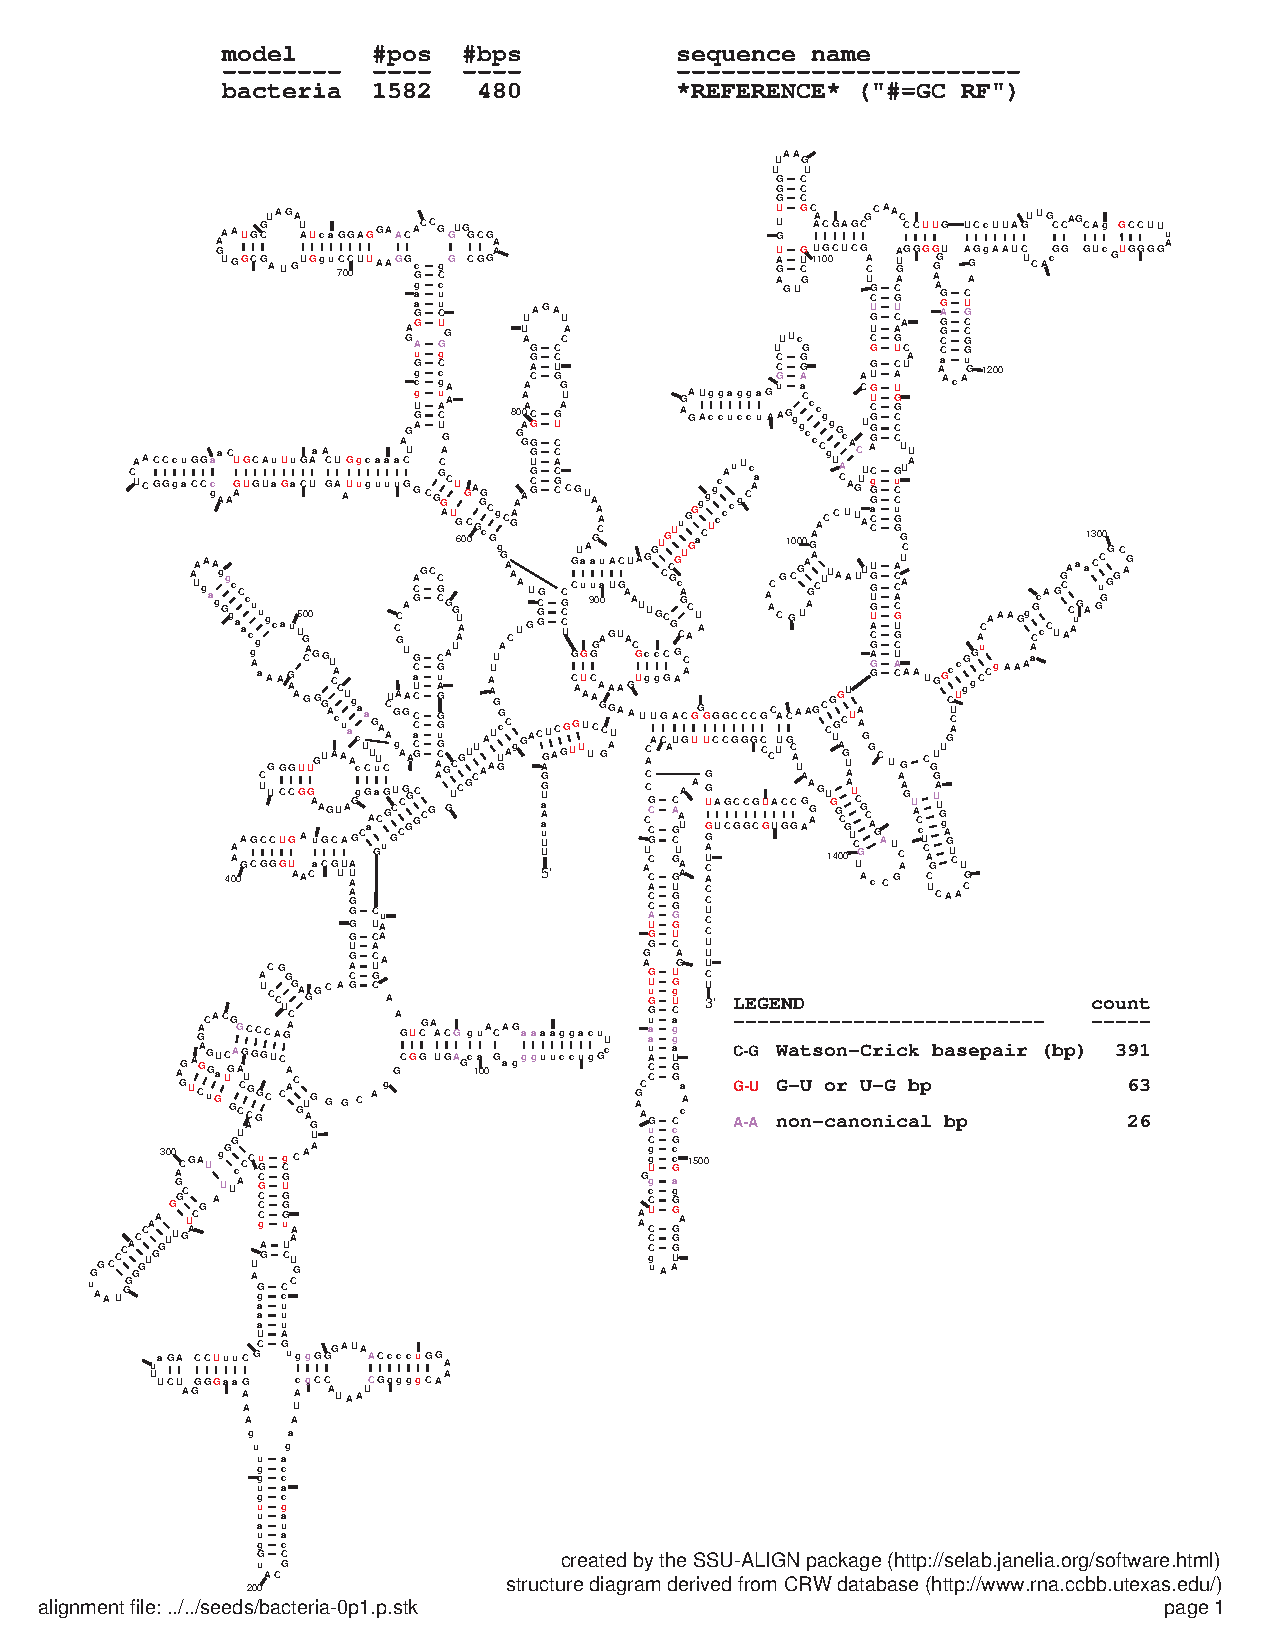
\includegraphics[height=8.5in]{Figures/bacteria-0p1-rf}
%\caption{Consensus sequence and structure of the default bacterial
%  model of \sft{SSU-align} 0.1}.
%\label{fig:bacseedrf}
%\end{figure}

Create a new directory and copy the bacterial seed alignment in
\prog{ssu-align-0.1/seeds/bacteria-0p1.stk}, the default parameters
file \prog{ssu-align-0.1/sa-0p1.params}, and the file
\prog{ssu-align-0.1/tutorial/partial.fa} there.

Let's say our 5' primer begins at consensus position 35 and our 3'
primer ends at position 397.  In practice, you'll have to manually
find your primer site and determine their positions on this consensus
structure. On the structure diagrams in section, every
hundredth residue is numbered, and every tenth residue is marked with
a tick mark, which should help you find the relevant positions.  If
you have a subsequence that exactly spans from one primer to another,
you can align it to the appropriate \textsc{ssu-align} model, then
number the consensus positions of that alignment with
\prog{esl-alimanip --num-rf} and examine the numbered alignment to
determine the primer positions.

\begin{srefaq}{If I'm creating a truncated model for sequences derived
    using specific primers, should I include the primer sequences
    within the new model or not?} You should include the primers
  because they will help the program correctly align each
  sequence. The primer sites are very highly conserved so they are
  simple for the program to correctly align and anchor the alignment
  of the rest of the sequence.
\end{srefaq}

For this example, the first step towards creating a truncated model is
to create a truncated seed alignment that only models between
consensus positions 35 and 397. We can do this with the
\prog{esl-alimanip} program using the full bacterial seed alignment as
input:

\user{esl-alimanip --start-rf 35 --end-rf 397 -o bac-35-397.stk bacteria-0p1.stk}

This command creates a new alignment called \prog{bac-35-397.stk} which
includes the subset of the columns from \prog{bacteria-0p1.stk} that lie
between consensus positions 35 and 397 inclusively.

The next step is to build a new model from this new alignment with
\textsc{infernal} 1.01's \prog{cmbuild} program. If this program is in
your path, you can execute it with \prog{cmbuild}, otherwise you'll
need to provide the full path. We will specify the name we want
to give the model with the \prog{-n} flag:

\user{cmbuild -n bac-35-397 --enone --gapthresh 0.8 bac-35-397.cm bac-35-397.stk}

\begin{srefaq}{Why did you specify \prog{--enone} and
    \prog{--gapthresh 0.8} as command-line flags to \prog{cmbuild}?}
    These are the recommended ``best-practice'' options for building
    models for SSU alignment. The \prog{--enone} flag tells the
    program to turn off entropy-weighting, a parameterization
    technique used to make CM homology search more sensitive
    \cite{Nawrocki07} but that seems slightly detrimental to CM
    alignment accuracy with SSU rRNA models. The \prog{--gapthresh
      0.8} flag tells the program to define any column that has less
    than 80\% gaps in the seed as a consensus column. Different values
    than 0.8 could be used here, but 0.8 empirically seems to yield
    good performance for SSU alignment. The \prog{--enone} and
    \prog{--gapthresh 0.8} flags were used to build
    \textsc{ssu-align}'s three default models in the \prog{seeds/}
    subdirectory of the package.
\end{srefaq}

Now you can begin using your new model \prog{bac-35-397.cm} to align
SSU sequences. You have two options.  You can either use your new
model by itself as the only model in an \prog{ssu-align} run, or you
can combine it with other models to create a multi-model file to use
with \prog{ssu-align}. The former option is recommended if you expect
all of your sequences to match the truncated model, that is, they all
are bacterial SSU subsequences that map close to the 35-397
region. I'll run through an example of this below. The latter option,
combining this model with others, is recommended if only a subset of
the sequences you will analyze are expected to match the truncated
model. In that case, the other models you combine the truncated model
with should span the diversity of the other sequences you expect in
your sequence dataset. (An example of using the multi-model file
\prog{\$SADIR/seeds/ssu3-0p1.cm} with \textsc{ssu-align} was
demonstrated at the beginning of this tutorial.)

For demonstration, we'll imagine all the sequences in our sequence
dataset are bacterial sequences that match near the 35-397 region. The
example sequence file \prog{partial.fa} includes 5 such sequences
derived from full length sequences in the bacterial seed alignment
\prog{\$SADIR/seeds/bacteria-0p1.fa} file. I artificially added 10
random residues to the 5\' and 3\' ends of the 5th sequence to
demonstrate that the program can trim residues it deems nonhomologous
to the model from the ends of the sequences before alignment.

\user{ssu-align bac-35-397.cm partial.fa single sa-0p1.params}

The program takes about 2 seconds to run. 

Take a look at the \prog{single.scores} file in the \prog{single/}
subdirectory:

\begin{sreoutput}
#                                                               best-matching model               
#                                                -------------------------------------------------
#     idx  sequence name                         model name   beg   end    CM sc   struct   HMM sc
# -------  ------------------------------------  ----------  ----  ----  -------  -------  -------
        1  00841::Escherichia_coli::J01695       bac-35-397     1   345   503.06    74.52   434.11
        2  00908::Myxococcus_xanthus::M34114     bac-35-397     1   355   481.88    77.81   416.33
        3  00886::Proteus_vulgaris::X07652       bac-35-397     1   345   500.24    72.28   432.49
        4  00225::Rickettsia_prowazekii::M21789  bac-35-397     1   327   478.08    60.64   422.20
        5  00020::Thermus_thermophilus::X07998   bac-35-397    11   350   447.37    67.84   394.77
\end{sreoutput}

Note how the alignment of the final sequence begins at position 11 and
ends at 350. The program truncated the first and last 10 nonhomologous
residues that I had manually added (that sequence is 360 residues long
in \prog{partial.fa}).
